\item[16] Consider the partial CPU datapath given here (found in hw5\_datapath.circ):

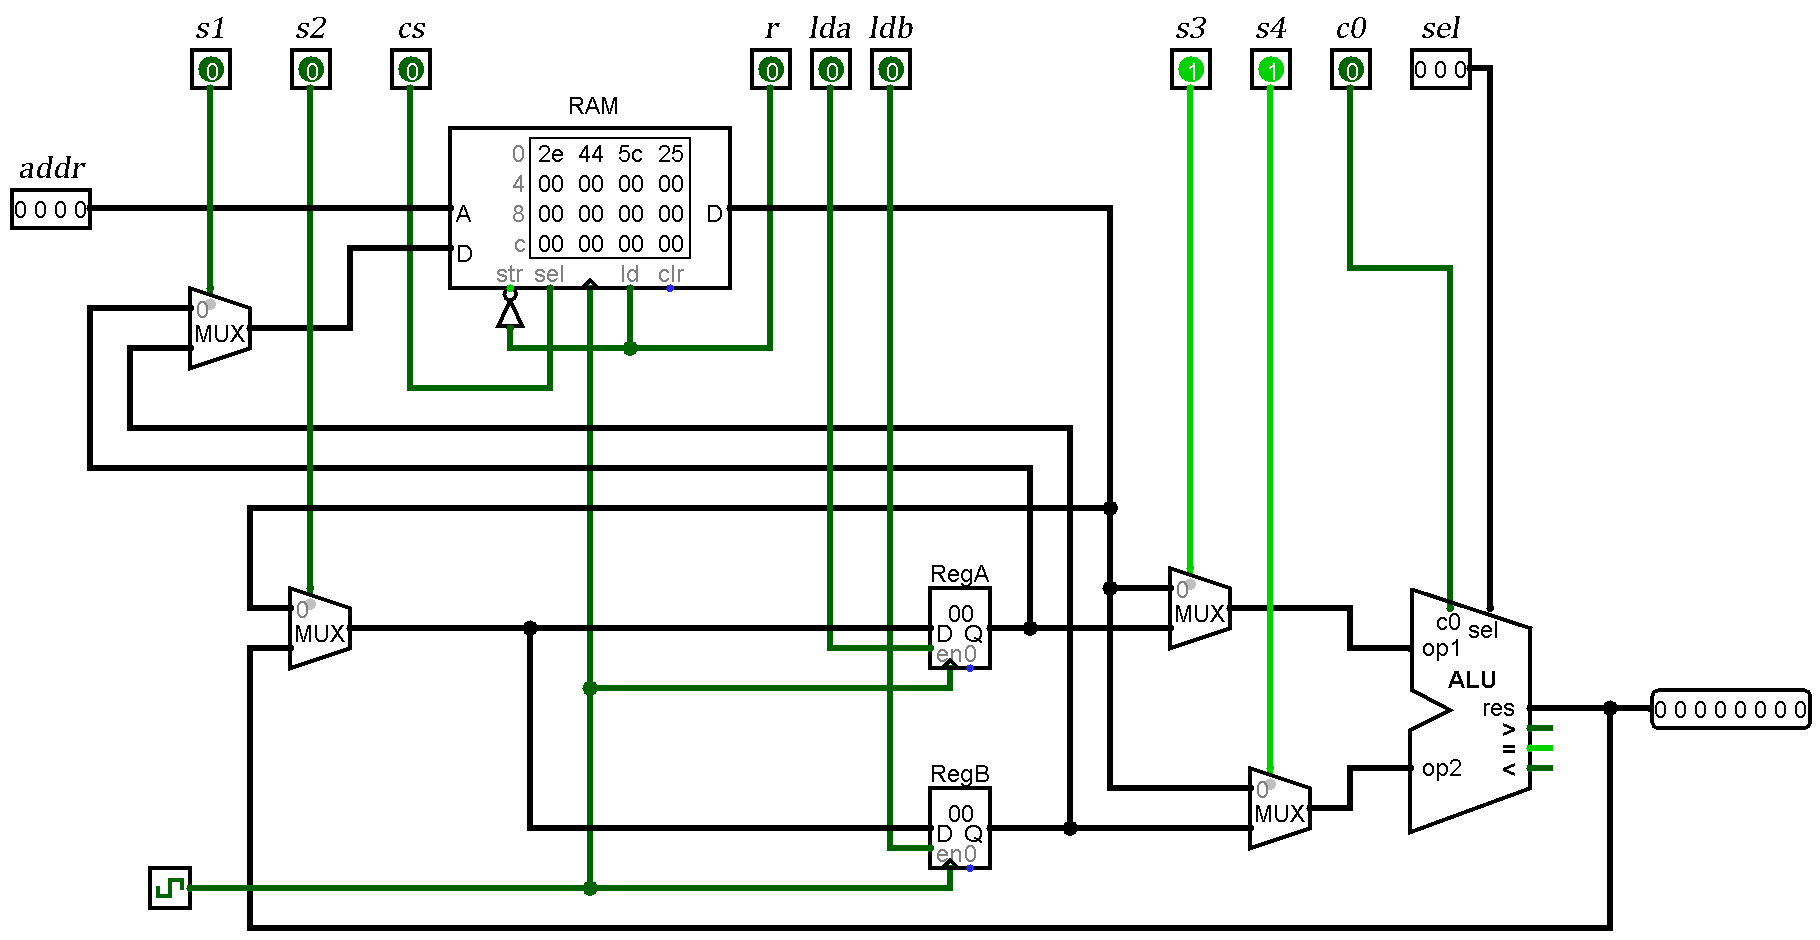
\includegraphics[width=15.5cm]{images/datapath_ex.png}

This datapath contains two 8-bit parallel load registers $A$ and $B$, a $2^4 \times 8$ RAM, and an 8-bit ALU with the function table below (NOTE - this is more or less the ALU described during the combinational logic lecture):

\begin{tabular}{c | l | c | l}
$sel$ & Function & $sel$ & Function \\
\hline
{\tt 0 0 0} & $res = op1 + c0$ & {\tt 1 0 0} & $res = c0$ \\
{\tt 0 0 1} & $res = op1 + op2 + c0$ & {\tt 1 0 1} & $res = op2 + c0$ \\
{\tt 0 1 0} & $res = op1 + \sim op2 + c0$ & {\tt 1 1 0} & $res = \sim op2 + c0$ \\
{\tt 0 1 1} & $res = op1 \land op2$ & {\tt 1 1 1} & $res = op1 \lor op2$ \\
\end{tabular}

For the next four parts of this question, you are to analyze the circuit to determine a sequence of appropriate assignments to every control input of the datapath (including $addr$), so that the final result of the required computation is stored into RAM at the specified address(es).

Some notes and guidelines:

\begin{itemize}
    \item Each 8-bit word in RAM is shown as hexadecimal (e.g. ${\tt2e}_{16} = 46_{10}$). Assume that negative numbers are represented using two's complement.
    \item Carefully study the diagram to observe the flow of 8-bit data values to/from registers and RAM.
    \item If any synchronous device is not involved in one of your intended operations, ensure that the device does not overwrite its contents during the operation (i.e. disable the device using $ld\_$ or $cs$ appropriately).
    \item In most cases, it is better practice to move needed values from RAM into the work registers for computation, and once a work register contains a result (or intermediate result), move it back to RAM unless you can use it again immediately.
    \item You may not overwrite your given initial data values in RAM.
    \item In completing the provided tables, write a 0 or 1 if the control input \textit{must} receive a 0 or 1 for the current operation. If the control input can receive either 0 or 1 without affecting the intended operation, write X (don't care).
    \item In the "Operation" column of the table, use register transfer notation to write a reasonable summary of the general operation.
    \item If testing your mini-program on the provided Logisim file, operations combining RAM retrieval with register storage and ALU \textit{might} require 2 clock cycles (not accurate to real-world microcontrollers, but it's the best Geoff could do in Logisim with the built-in RAM and register devices and this datapath configuration). Make sure your register load control is only active on the second clock cycle.
\end{itemize}

\newpage

  \begin{question}{(a)}[4]
  \item[4] Assume that $RAM\left[0\right]$ contains $46_{10}$, $RAM\left[1\right]$ contains $68_{10}$, $RAM\left[2\right]$ contains $92_{10}$, and $RAM\left[3\right]$ contains $37_{10}$. Other entries are unknown and can be overwritten. Determine a sequence of control input assignments to perform $(46 + 68) \uparrow (92 - 37)$ and store the final result into $RAM\left[15\right]$. The first operation is completed for you as an example.
  {\color{NavyBlue}
  \begin{Questions}
  \begin{tabular}{p{5cm} | c | c | c | c | c | c | c | c | c | c | c}
  Operation & $\, addr \,$ & $\, s_1 \,$ & $\, s_2 \,$ & $\, cs \,$ & $\, r \,$ & $\, lda \,$ & $\, ldb \,$ & $\, s_3 \,$ & $\, s_4 \,$ & $\, c0 \,$ & $\, sel \,$ \\
  \hline
  $RegA \leftarrow RAM\left[0\right]$ & 0000 & X & 0 & 1 & 1 & 1 & 0 & X & X & X & XXX \\
  $RegB \leftarrow RegA + RAM\left[1\right]$ & 0001 & X & 1 & 1 & 1 & 0 & 1 & 1 & 0 & 0 & 001 \\
  $ RAM\left[4\right] \leftarrow RegB$ & 0100 & 1 & X & 1 & 0 & 0 & 0 & X & X & X & XXX \\
  $RegB \leftarrow RAM\left[3\right]$ & 0011 & X & 0 & 1 & 1 & 0 & 1 & X & X & X & XXX \\
  $RegB \leftarrow RAM\left[2\right] + \lnot RegB$ + 1& 0010 & X & 1 & 1 & 1 & 0 & 1 & 0 & 1 & 1 & 010 \\
  $RegB \leftarrow RAM\left[4\right] \land RegB$ & 0100 & X & 1 & 1 & 1 & 0 & 1 & 0 & 1 & X & 011 \\
  $RegB \leftarrow \lnot RegB$ & XXXX & X & 1 & 0 & X & 0 & 1 & X & 1 & 0 & 110 \\
  $ RAM\left[15\right] \leftarrow RegB$ & 1111 & 1 & X & 1 & 0 & 0 & 0 & X & X & X & XXX \\
  \end{tabular}
  \end{Questions}
  }
  \item[4] Assume that $RAM\left[3\right]$ contains $73_{10}$. Other entries are unknown and can be overwritten. Determine a sequence of control input assignments, so that $-70_{10}$ is stored into $RAM\left[15\right]$.
  {\color{NavyBlue}
 \begin{Questions}
  \begin{tabular}{p{4.3cm} | c | c | c | c | c | c | c | c | c | c | c}
  Operation & $\, addr \,$ & $\, s_1 \,$ & $\, s_2 \,$ & $\, cs \,$ & $\, r \,$ & $\, lda \,$ & $\, ldb \,$ & $\, s_3 \,$ & $\, s_4 \,$ & $\, c0 \,$ & $\, sel \,$ \\
  \hline
  $RegA \leftarrow RAM\left[3\right]$ & 0011 & X & 0 & 1 & 1 & 1 & 0 & X & X & X & XXX \\
  $RegB \leftarrow 0 $ & XXXX & X & 1 & 0 & X & 0 & 1 & X & X & 0 & 100 \\
  $RegA \leftarrow RegA + \lnot RegB$ & XXXX & X & 1 & 0 & X & 1 & 0 & 1 & 1 & 0 & 010 \\
  $RegA \leftarrow RegA + \lnot RegB$ & XXXX & X & 1 & 0 & X & 1 & 0 & 1 & 1 & 0 & 010 \\
  $RegB \leftarrow RegA + \lnot RegB$ & XXXX & X & 1 & 0 & X & 0 & 1 & 1 & 1 & 0 & 010 \\
  $RegB \leftarrow \lnot RegB + 1$ & XXXX & X & 1 & 0 & X & 0 & 1 & X & 1 & 1 & 110 \\
  $ RAM\left[15\right] \leftarrow RegB$ & 1111 & 1 & X & 1 & 0 & 0 & 0 & X & X & X & XXX \\
  \end{tabular}
 \end{Questions}
 }
 \item[4] Assume that $RAM\left[0\right]$ contains $16_{10}$, $RAM\left[1\right]$ contains $38_{10}$, and $RAM\left[2\right]$ contains $61_{10}$. Other entries are unknown and can be overwritten. Determine a sequence of control input assignments, so that $(38 + 61) \text{ mod } 16$ is stored into $RAM\left[15\right]$.\\
 {\color{NavyBlue}
 \begin{Questions}
  \begin{tabular}{p{4.7cm} | c | c | c | c | c | c | c | c | c | c | c}
  Operation & $\, addr \,$ & $\, s_1 \,$ & $\, s_2 \,$ & $\, cs \,$ & $\, r \,$ & $\, lda \,$ & $\, ldb \,$ & $\, s_3 \,$ & $\, s_4 \,$ & $\, c0 \,$ & $\, sel \,$ \\
  \hline$RegA \leftarrow RAM\left[2\right]$ & 0010 & X & 0 & 1 & 1 & 1 & 0 & X & X & X & XXX \\
  $RegA \leftarrow RegA + RAM\left[1\right]$ & 0001 & X & 1 & 1 & 1 & 1 & 0 & 1 & 0 & 0 & 001 \\
  $RegB \leftarrow RAM\left[0\right]$ & 0000 & X & 0 & 1 & 1 & 0 & 1 & X & X & X & XXX \\
  $RegA \leftarrow RegA + \lnot RegB$ + 1& XXXX & X & 1 & 0 & X & 1 & 0 & 1 & 1 & 1 & 010 \\
  $RegA \leftarrow RegA + \lnot RegB$ + 1& XXXX & X & 1 & 0 & X & 1 & 0 & 1 & 1 & 1 & 010 \\
  $RegA \leftarrow RegA + \lnot RegB$ + 1& XXXX & X & 1 & 0 & X & 1 & 0 & 1 & 1 & 1 & 010 \\
  $RegA \leftarrow RegA + \lnot RegB$ + 1& XXXX & X & 1 & 0 & X & 1 & 0 & 1 & 1 & 1 & 010 \\
  $RegA \leftarrow RegA + \lnot RegB$ + 1& XXXX & X & 1 & 0 & X & 1 & 0 & 1 & 1 & 1 & 010 \\
  $RegA \leftarrow RegA + \lnot RegB$ + 1& XXXX & X & 1 & 0 & X & 1 & 0 & 1 & 1 & 1 & 010 \\
  $ RAM\left[15\right] \leftarrow RegA$ & 1111 & 0 & X & 1 & 0 & 0 & 0 & X & X & X & XXX \\
    
  \end{tabular}
 \end{Questions}
 }
 \item[4] All entries are unknown and can be overwritten. Store $00_{16}$ into $RAM\left[0\right]$ and $RAM\left[2\right]$, and store ${\tt ff}_{16}$ into $RAM\left[1\right]$ and $RAM\left[3\right]$.\\
 {\color{NavyBlue}
 \begin{Questions}
  \begin{tabular}{p{4.3cm} | c | c | c | c | c | c | c | c | c | c | c}
  Operation & $\, addr \,$ & $\, s_1 \,$ & $\, s_2 \,$ & $\, cs \,$ & $\, r \,$ & $\, lda \,$ & $\, ldb \,$ & $\, s_3 \,$ & $\, s_4 \,$ & $\, c0 \,$ & $\, sel \,$ \\  

  \hline
  $RegB \leftarrow 0 $ & XXXX & X & 1 & 0 & X & 0 & 1 & X & X & 0 & 100 \\
  $ RAM\left[0\right] \leftarrow RegB$ & 0000 & 1 & X & 1 & 0 & 0 & 0 & X & X & X & XXX \\
  $ RAM\left[2\right] \leftarrow RegB$ & 0010 & 1 & X & 1 & 0 & 0 & 0 & X & X & X & XXX \\
  $RegB \leftarrow \lnot RegB $ & XXXX & X & 1 & 0 & X & 0 & 1 & X & 1 & 0 & 110 \\
  $ RAM\left[1\right] \leftarrow RegB$ & 0001 & 1 & X & 1 & 0 & 0 & 0 & X & X & X & XXX \\
  $ RAM\left[3\right] \leftarrow RegB$ & 0011 & 1 & X & 1 & 0 & 0 & 0 & X & X & X & XXX \\
  \end{tabular}
 \end{Questions}
 }
 \vspace{2.0cm}
 
You may have noticed that some of the operations you are asked to do (e.g. NAND), are not directly supported by the ALU. It is the job of the \textbf{compiler} to turn a high-level instruction into a sequence of ALU-supported low-level instructions that produce the required result. Thank you for your effort in this course, good luck with the rest of your studies!

\end{question}